        \subsection{history}

\begin{frame}\frametitle{introduction}\framesubtitle{release of digital technology --- production}
	\begin{columns}
		\column{5cm}
			\begin{scriptsize}
			\begin{table}
					\begin{tabular}{lr}
					\hline
						\textbf{Product} & \textbf{Year} \\
					\hline%
					\uncover<1->{%
						\textbf{Sound Synthesis} &            \\
						
						NED Synclavier Synthesizer/Sampler &       1979 \\
						
						Fairlight CMI Synthesizer/Sampler &       1979 \\
						
						Linn LM-1 Drumcomputer/Sampler	&				1980	\\
						
						E-MU Emulator I Sampling Keyboard &       1981 \\
						
						\only<1>{\textcolor{blue}}{Yamaha DX-7 Syntheziser} &       1983\vspace{1mm}\\
						
					}%		
					\uncover<2->{%
						\textbf{Sound Processing/Effects} &            \\
						
						Lexicon Delta-T 101 Digital Delay & 1971 \\
						
						EMT 250 Digital Reverberation & 1976 \\
						
						\only<2>{\textcolor{blue}}{Lexicon L224 Digital Reverberation} &       1978\vspace{1mm} \\
							
					}%	
					\uncover<3->{%
						\textbf{Sound Editing} &            \\
						
						Sony DAE-1100 Digital Audio Editor &       1980 \\
						
						\only<3>{\textcolor{blue}}{Sony DAE-3000 Digital Audio Editor} &       1987 \\
		
						Sonic Solutions Harddisk Editing &       1988\vspace{1mm}\\
						
					}%
					\uncover<4->{%
						\textbf{Other} &            \\
						
						\only<4>{\textcolor{blue}}{MIDI Standard}	&			1983		\\
					\hline
					}
					\end{tabular}  
			\end{table}
			\end{scriptsize}
		\column{3cm}
			\only<1>{
				\begin{figure}
					\centering
					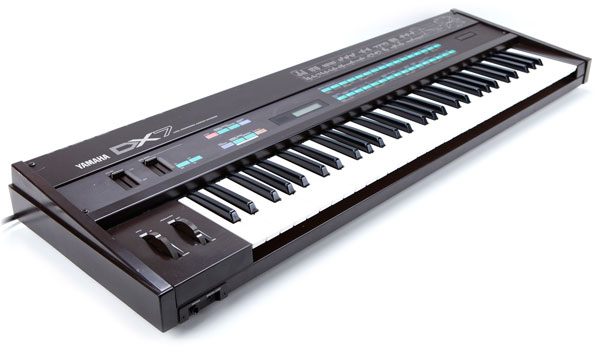
\includegraphics[scale=.3]{graph/yamaha_dx7}
				\end{figure}
			}
			\only<2>{
				\begin{figure}
					\centering
					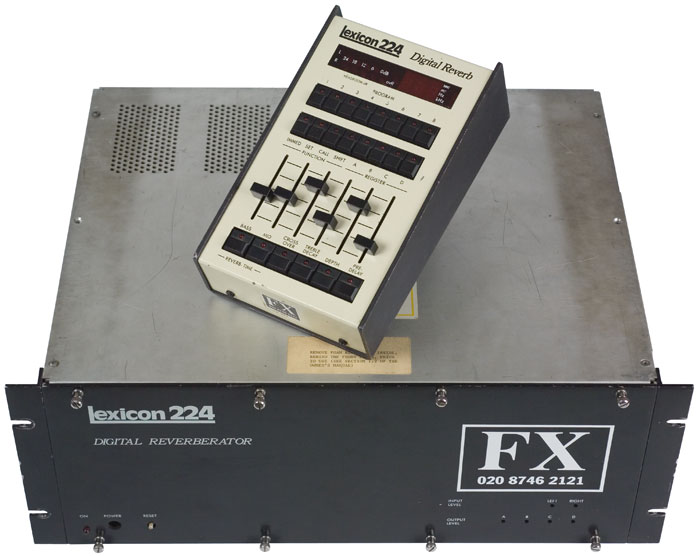
\includegraphics[scale=.15]{graph/lexicon224}
				\end{figure}
			}
			\only<3>{
				\begin{figure}
					\centering
					\includegraphics[scale=.4]{graph/sony_DAE3000}
				\end{figure}
			}
			\only<4>{
				\begin{figure}
					\centering
					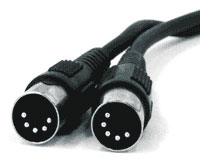
\includegraphics[scale=.5]{graph/midi_cable}
				\end{figure}
			}
	\end{columns}
\end{frame}

\begin{frame}\frametitle{introduction}\framesubtitle{release of digital technology --- storage \& consumer}
	\begin{columns}
		\column{5cm}
			\begin{scriptsize}
			\begin{table}
				\begin{tabular}{lr}
				\hline
					\textbf{Digital Storage} & \textbf{Year} \\
				\hline%
				\uncover<1->{%
					\textbf{Professional} &            \\
					PCM-1600 (U-matic)	&			1978	\\
					PCM-1 (Betamax)	&			1978	\\
					
					Digital Multitrack (3M, Sony)	&			1978	\\
					
					Alesis ADAT &       1991 \\
					
					\only<1>{\textcolor{blue}}{Tascam DA-88} &       1993\vspace{1mm}  \\
				}%
				\uncover<2->{%
					\textbf{Consumer} &            \\
					\only<2>{\textcolor{blue}}{Compact Disc} &       1982/83\\
					Digital Audio Tape (DAT) &       1987\\
					MiniDisc &       1991\\
					Digital Compact Cassette &       1992\\
					DVD-Video & 	1997\\
					DVD-Audio & 1999\\
					SACD & 1999\\
					\hline
				}
				\end{tabular}  
			\end{table}
			\end{scriptsize}
		\column{3cm}
			\only<1>{
				\begin{figure}
					\centering
					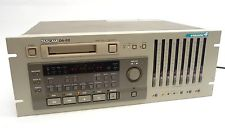
\includegraphics[scale=1.3]{graph/tascam_da88}
				\end{figure}
			}
			\only<2>{
				\begin{figure}
					\centering
					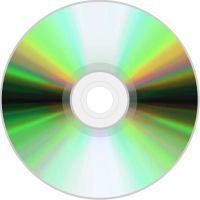
\includegraphics[scale=.3]{graph/compact_disc}
				\end{figure}
			}
	\end{columns}
\end{frame}


\begin{frame}{introduction}{reasons for digital equipment}
	\begin{itemize}
        \item   \textbf{storage}:
            \begin{itemize}
                \item   lossless copying and archiving of digital content
            \end{itemize}
        \pause
        \item   \textbf{editing \& processing} 
            \begin{itemize}
                \item   splicing of recordings
                \item   fast convolution
                \item   granular processing/time-stretching/pitch-shifting
            \end{itemize}
        \pause
		\item	\textbf{technical characteristics}
			\begin{itemize}
				\item	SNR, distortion, transfer functions, ...
			\end{itemize}
            \bigskip
        \pause
        \item   \textbf{dropping prices} for digital hardware and software (compared to analogue equipment)
    \end{itemize}
\end{frame}

\begin{frame}{introduction}{current trends \& developments}
	\begin{itemize}
		\item	\textbf{resolution and data rates}
			\begin{itemize}
				\item	higher bit resolution and sample rates?
				\item	compression formats
			\end{itemize}
		\pause
		\item	\textbf{audio formats}
			\begin{itemize}
				\item	multichannel \& WFS, 3D acoustics in general
                \item   object-based audio
			\end{itemize}
		%\pause
		%\item	\textbf{further digitization and improvements of equipment}
			%\begin{itemize}
				%\item	microphones \& speakers
				%\item	(remote control of) DSP-enabled systems
				%\item	converters \& storage
			%\end{itemize}
		%\pause
		%\item	\textbf{transmission and distribution channels}
			%\begin{itemize}
				%\item	streaming on demand
				%\item	subscription models
			%\end{itemize}
		\pause
		\item	\textbf{production environments}
			\begin{itemize}
				\item	online collaboration/musicianship
                \item   machine musicianship
			\end{itemize}
		\pause
		\item	\textbf{software}
			\begin{itemize}
				\item	machine listening:  music recommendation systems, etc.
				\item	signal- and user-adaptive audio production software
				\item	computer-aided editing, composition, and performance systems
                \item   interactive and creative audio consumer software
			\end{itemize}
	\end{itemize}
\end{frame}

